\documentclass{article}

\usepackage[utf8]{inputenc}
\usepackage{graphicx}
\usepackage[a4paper,left=20mm,right=20mm,top=20mm,bottom=20mm]{geometry}

\begin{document}

\begin{center}
    \section*{INE5415 - Teoria da Computação (2015/1)}
    \textbf{Trabalho 1 - Máquinas de Turing \\
    Antonio Luiz Rosa Teixeira, Gustavo Zambonin}
\end{center}

\subsection*{Questão 1}
\textit{L(M)} = \{$0^{2^{n}}$ p/ $n \geq 0$\}
\begin{itemize}
    \item \textbf{Descrição do funcionamento}: A máquina, primeiramente, marca
    um símbolo vazio no começo da fita para que saiba o seu início. Depois,
    conta os zeros aos pares, marcando-os e voltando ao início da fita. Se
    ainda existirem zeros desmarcados, o processo se repetirá, mas apenas
    marcando um a cada quatro zeros, e assim por diante, respeitando as
    potências de 2. O processamento da máquina força o estado de rejeição na
    primeira marcação dos zeros se não encontrar uma entrada de tamanho $2^{n}$.
    \item \textbf{Codificação da máquina}: \\
    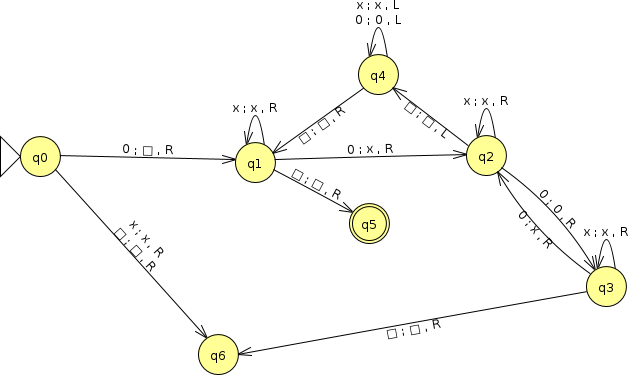
\includegraphics[scale=0.5]{questao1_ss.png}
    \item \textbf{Testes realizados}: \\ \\
    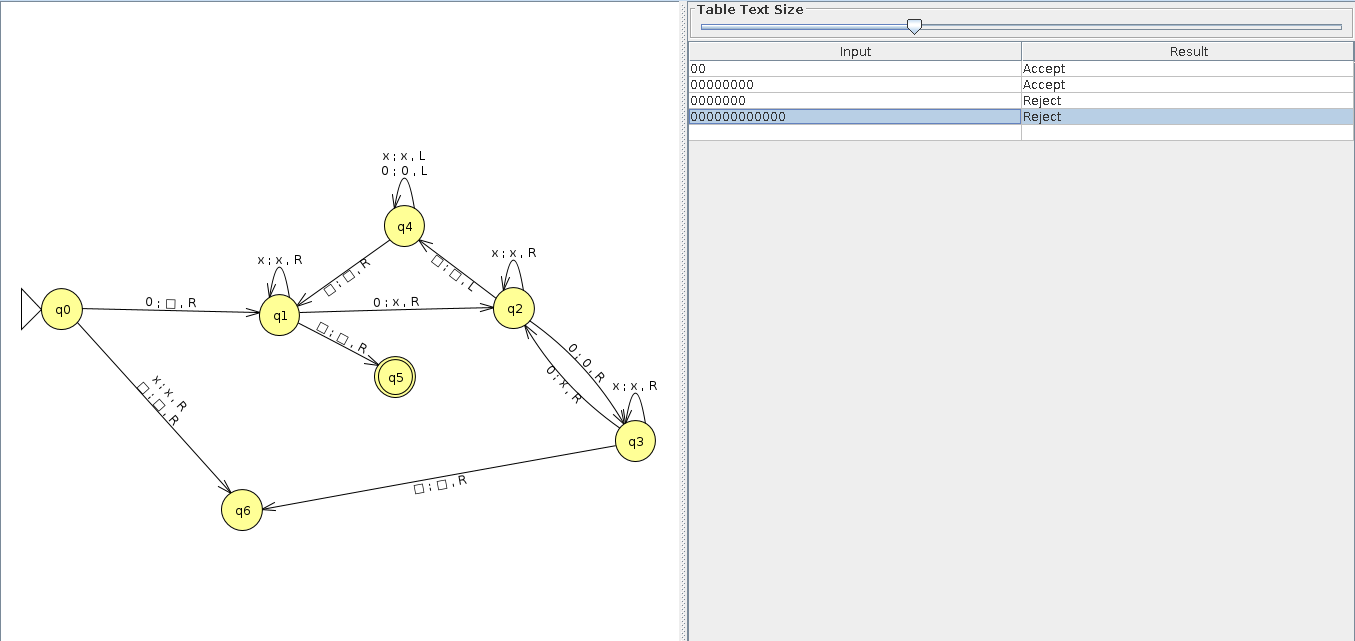
\includegraphics[width=\textwidth]{questao1_inputs.png}
\end{itemize}
\newpage

\subsection*{Questão 2}
\textit{L(M)} = \{$a^{i}b^{j}c^{k}\ \vert\  i \times j = k $ e $i,j,k \geq 1$\}
\begin{itemize}
    \item \textbf{Descrição do funcionamento}: A máquina marca um A e a
    quantidade inteira de letras B, e a mesma quantidade de letras C, fazendo
    uma operação similar à soma de multiplicações triviais. Ao final da marcação
    de letras C, as letras B são desmarcadas e a próxima letra A é marcada, e
    assim por diante. Se a multiplicação não apresentar seu resultado correto,
    lembrando que todas as letras precisam aparecer pelo menos uma vez, a
    máquina rejeitará a entrada.
    \item \textbf{Codificação da máquina}: \\
    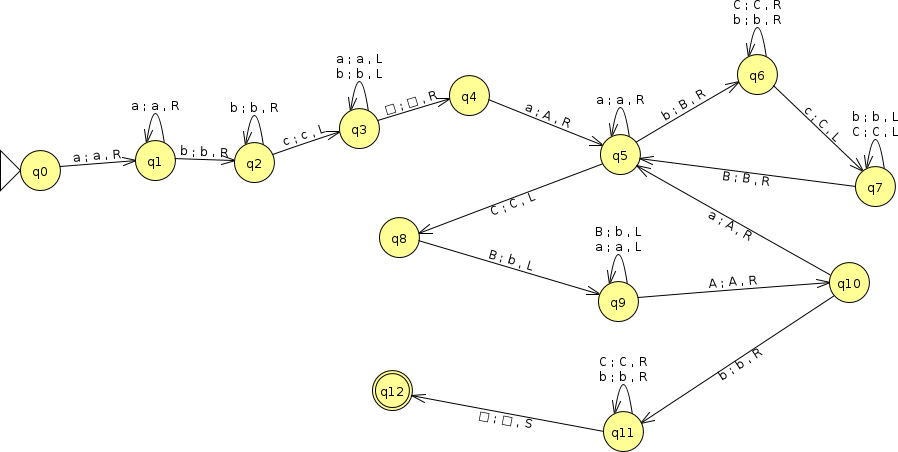
\includegraphics[scale=0.5]{questao2_ss.png}
	\item \textbf{Testes realizados}: \\ \\
    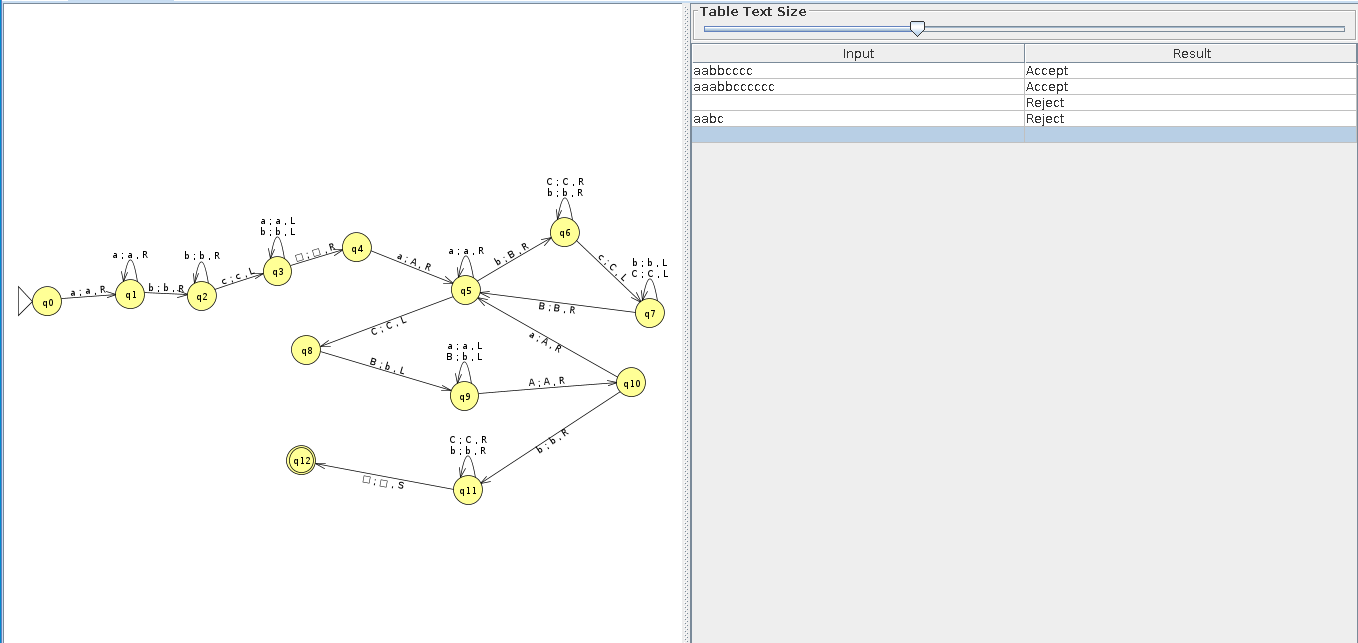
\includegraphics[width=\textwidth]{questao2_inputs.png}
\end{itemize}
\newpage

\subsection*{Questão 3}
\textit{L(M)} = \{$\#x_{1}\#x_{2}\#...\#x_{n}\  \vert\  x_{i} \in \Sigma =
\{0,1\}^{*}$ e $x_{i} \neq x_{j}$ para cada $i \neq j$\}
\begin{itemize}
    \item \textbf{Descrição do funcionamento}: A máquina compara $x_i$ e $x_j$,
    $\forall i\neq j$, exceto pela palavra vazia, garantida no início do
    procedimento. Após esta garantia, um $x_i$ é fixado e comparado com
    $x_{i+1}$, $x_{i+2}$, ..., $x_n$. Depois do final dessa comparação, a
    próxima subpalavra, $x_{i+1}$, é fixada e comparada com os elementos
    posteriores, separados pelo \#, até que este não seja mais encontrado na
    entrada, significando o fim da mesma.
    \item \textbf{Codificação da máquina}: \\
    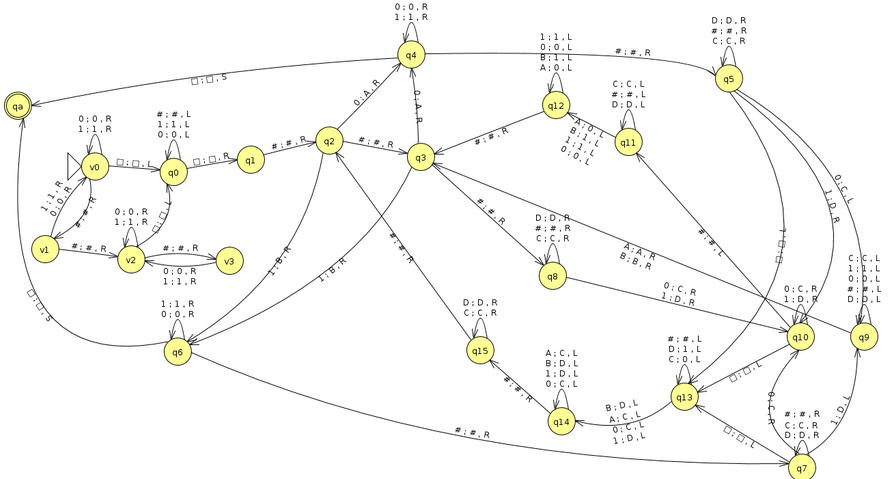
\includegraphics[width=\textwidth]{questao3_ss.png}
    \item \textbf{Testes realizados}: \\ \\
    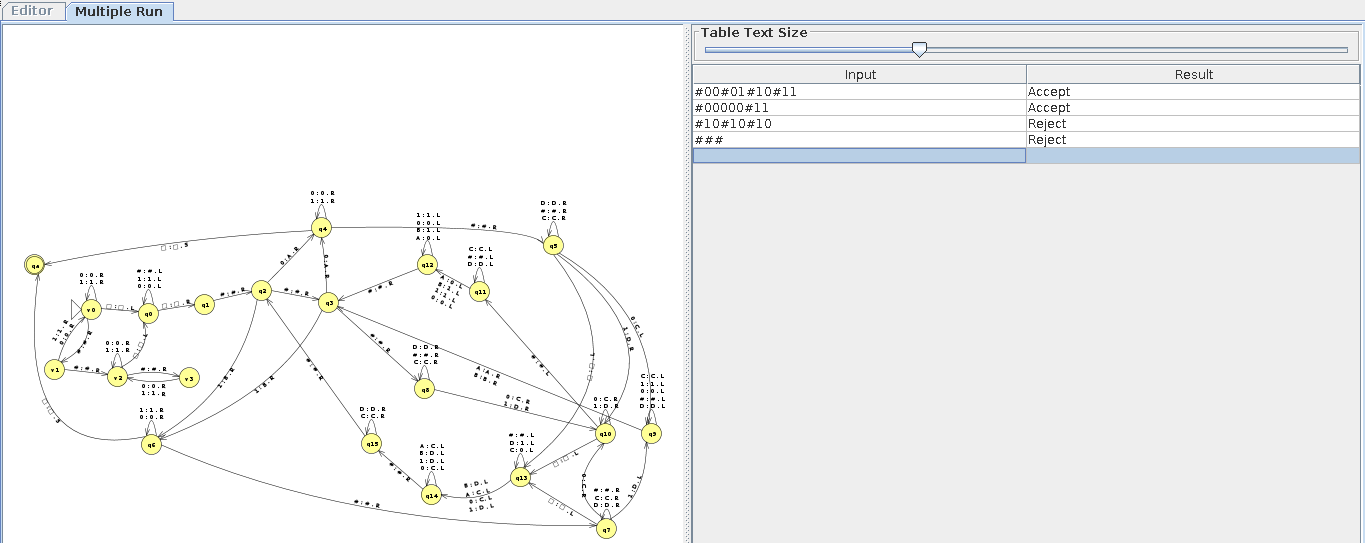
\includegraphics[width=\textwidth]{questao3_inputs.png}
\end{itemize}

\end{document}
